\section{System Analysis}
\subsection{Individuals}
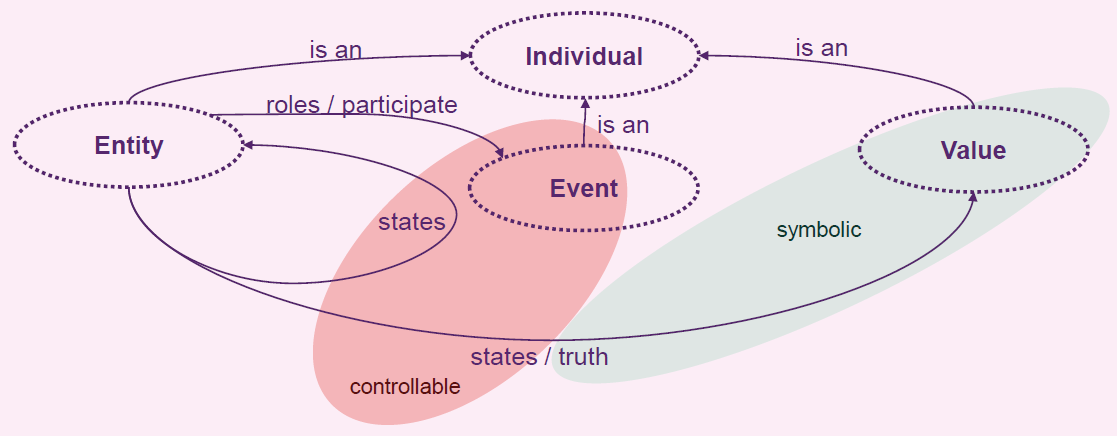
\includegraphics[width=\linewidth]{./img/value_overview.png}
\textbf{Events:}
\begin{itemize}
    \item Individual Happening, taking place at some particular point in time
    \item \textit{E.g. User-Action}
\end{itemize}
\textbf{Entities:}
\begin{itemize}
    \item Individual that persists over time and can change its properties and states.
    \item May initiate events
    \item May cause spontaneous changes to their own states
    \item May be passive
    \item \textit{E.g. Person}
\end{itemize}
\textbf{Values:}
\begin{itemize}
    \item Intangible (nicht greifbar) individual that exists outside time and space
    \item Not subject to change
    \item \textit{E.g. Körpergrösse}
\end{itemize}

\section{Software Design}
\subsection{Categories of Objects}
\textbf{Entity}
\begin{itemize}
    \item Express system information
    \item Typically persistent in nature
    \item Identity is important to distinguish entity objects
\end{itemize}
\textbf{Service}
\begin{itemize}
    \item Represent system activities
    \item Distinguished by their behaviour rather than their state
\end{itemize}
\textbf{Values}
\begin{itemize}
    \item Interpreted content is the dominant characteristic
    \item Transient and do not have significant enduring indentity
\end{itemize}
\textbf{Task}
\begin{itemize}
    \item Represent system activities
    \item Have an element of identity and state
\end{itemize}

\section{Object Aspects}
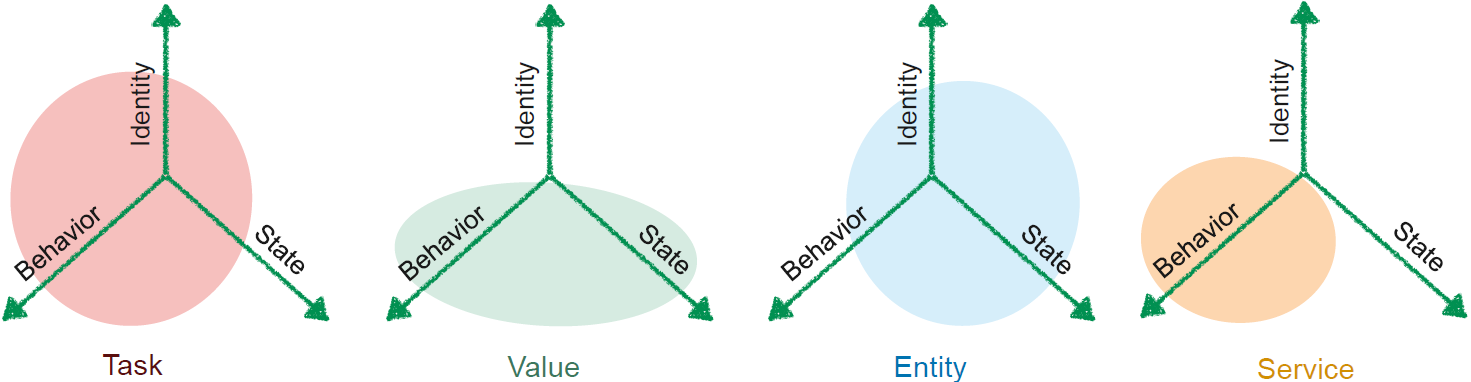
\includegraphics[width=\linewidth]{./img/object_aspects.png}

\section{Value Objects}
\begin{itemize}
    \item Usually do not appear in UML class diagrams (except attribute type)
    \item Model fine-grained information
    \item Contain repetitive common code
    \item Used to add meaning to primitive value types
    \item Ensure type safety
    \item \textit{E.g. IBAN Type Object (10 digits, checksum)}
\end{itemize}

\section{Value patterns}
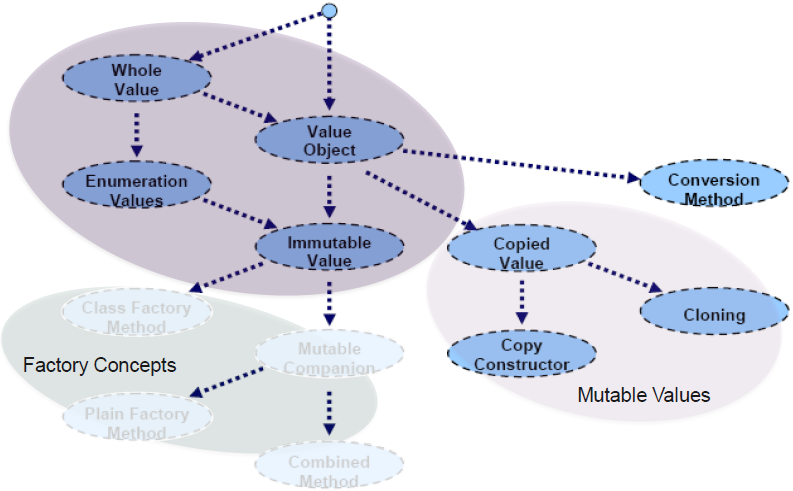
\includegraphics[width=\linewidth]{./img/value_pattern_overview.png}

\subsection{Whole Value}
\subsubsection{Problem}
\begin{itemize}
    \item Plain integers and floating-point numbers are not very useful as domain values
    \item Errors in dimension and intent communication should be addressed at complile time
    \item How can you represent primitive quantities from your proble domain without loss of meaning?
\end{itemize}
\subsubsection{Solution}
Express the type of the quantity as a Value Class.\\ 
\begin{itemize}
    \item Recovers the loss of meaning and checking by providing a \textbf{dimension} and \textbf{range}
    \item Wraps simple types or attribute stes
    \item Disallows inheritance to avoid slicing
    \item \textit{E.g. Year, Month, Day Classes for Dates}
\end{itemize}
\begin{lstlisting}
public final class Date {
    public Date(Year year, Month month, Day day) { ... }
}
\end{lstlisting}

\subsection{Value Object / Value Class}
\subsubsection{Problem}
\begin{itemize}
    \item Comparison, indexing and ordering should not rely on objects identity but its content
    \item How do you define a class to represent values in your system?
\end{itemize}
\subsubsection{Solution}
Override methods in Object whose action should be related to content and not identity and implement serializable.\\
\begin{itemize}
    \item Override Object's methods who define equality
    \item Java
    \begin{itemize}
        \item \textit{equals(Object other)}
        \item \textit{hashCode()}
        \item implement \textit{Serializable / toString()} if appropriate
    \end{itemize}
    \item TypeScript
    \begin{itemize}
        \item \textit{equals(other: Object)}
        \item implement \textit{toString()} if appropriate
    \end{itemize}
    \item Overriding \textit{toString()} can help using your Value Object
\end{itemize}

\subsection{Conversion Method}
\subsubsection{Problem}
\begin{itemize}
    \item Values are strongely informational objects without a role for separate identity
    \item Often Value Objects are somehow related but cannot be used directly without conversion
    \item How could you use different, related Value Objects together without depending on underlying primitive type?
\end{itemize}
\subsubsection{Solution}
Provide type conversion methods responsible for converting Value Objects into related formats.
\begin{itemize}
    \item Provide a constructor which converts between types\\\textit{String(char[] value)}
    \item Or create a conversion instance method that converts to other type \\\textit{Date.toOtherType()}
    \item Or create a \textbf{Class Factory Method} with conversion characteristics \\\textit{Date.from(Instant i)}
\end{itemize}

\subsection{Immutable Value}
\subsubsection{Problem}
\begin{itemize}
    \item A value exists outside time and space and is not subject to change
    \item Avoid side effect problems when sharing Value Objects
    \item Sharing values across Threads requires thread safety
    \item Values are often threaded as key for associative tables
    \item How can you share Value Objects and guarantee no side effect problems?
\end{itemize}
\subsubsection{Solution}
Set the internal state of the Value Class object at construction and allow no modifications.\\ 
\begin{itemize}
    \item Declare all fields private final
    \item Mark class as final
    \item No Syncrhonization needed
\end{itemize}

\subsection{Enumeration Values}
\subsubsection{Problem}
\begin{itemize}
    \item A fixed range of values should be typed \textit{e.g. months}
    \item Using just int constants doesn't help
    \item Whole Value is only half the solution; range should be constant
    \item How can you represent a fixed set of constant values and preserve type safety?
\end{itemize}
\subsubsection{Solution}
Treat each constant as Whole Value instance declaring it public.
\begin{itemize}
    \item Implement a Whole Value and declare the Enumeration Values as \textit{public readonly} fields
    \item Prevent inadvertently changing the constants
    \item Pattern is built in (enum)
\end{itemize}

\subsection{Copied Value and Cloning}
\subsubsection{Problem}
\begin{itemize}
    \item Values should be modifiable without changing the origins internal state
    \item How can you pass a modifiable Value Object into and out of methods without permitting callers or called methods to affect the original object?
\end{itemize}
\subsubsection{Solution}
Implement Cloneable interface to be used whenever a value object needs to be returned or passed as a parameter.
\begin{itemize}
    \item Clone every Value Object leaked across boundaries (parameters / return values)
    \item May result in immense object creation overhead (cloning is expensive)
    \item Imitates \textit{call-by-value} and \textit{return-by-value}
\end{itemize}

\subsection{Copy Constructor}
\subsubsection{Problem}
\begin{itemize}
    \item Within Value Objects we often know exactly what to copy
    \item How can objects be copied without the need of implementing a clone method?
\end{itemize}
\subsubsection{Solution}
Provide a way to construct an object based on another instance with exactly the same type.
\begin{itemize}
    \item Declare the class \textit{final} and derive from Object only
    \item Create a copy constructor, which consumes an instance with same type
\end{itemize} 
\begin{lstlisting}
public final class Date {
    public Date(Date other) {
        // ... 
        this.year = new Year(other.year);
    }
}
\end{lstlisting}

\subsection{Class Factory Method / Simple Factory}
\subsubsection{Problem}
\begin{itemize}
    \item Construction of Value Objects may be expensive
    \item Different construction logic is required which may result in huge amount of constructors
    \item How can you simplify and potentially optimize construction of Value Objects in expressions without introducing new intrusive expressions?
\end{itemize}
\subsubsection{Solution}
Provide static methods to be used instead of ordinary constructors. The methods return either newly created Value Objects or cached Objects.
\begin{itemize}
    \item Declare one or more creation method on the class
    \item Define constructors \textit{private}, they are invoked by Class Factory Method
    \item The static methods could also contain caching mechanisms
\end{itemize}
\begin{lstlisting}
public final class Year {
    public static Year of(int value) {
        return new Year(value);
    }
    private Year(int value) { this.value = value; }
}
\end{lstlisting}

\subsection{Mutable Companion}
\subsubsection{Problem}
\begin{itemize}
    \item We need to calculate with alues \textit{e.g. 15 working days after exam}
    \item How can you simplify complex construction of an immutable value?
\end{itemize}
\subsubsection{Solution}
Implement a companion class that supports modifier methods and acts as a factory for immutable Value Objects.
\begin{itemize}
    \item Factory Object for immutable values
    \item Neither a subtype nor a supertype of the Immutable Value
\end{itemize}
\begin{lstlisting}
public final class YearCompanion {
    private int value;
    public YearCompanion(Year toModify) { this.value = toModify.getValue(); }
    /* modifying methods */
    public Year asValue() { /* Factory Method */
        return Year.of(value);
    }
}
\end{lstlisting}

\subsection{Relative Values}
\subsubsection{Problem}
\begin{itemize}
    \item Value Objects are compared by their state, not their identity
    \item Relative comparison between Value Objects for appropriate values should be provided
    \item How can a Value Obejct be compared against others in a typed way?
\end{itemize}
\subsubsection{Solution}
Implement the responsibility for comparison between Value Objects by deriving from \textit{Comparable} interface.
\begin{itemize}
    \item Override-Overload Method Pair: (\textit{compareTo(T other)} and \textit{equals(T other)})
    \item Bridge Method: Provide a Method for \textit{equals(Object other)} and forward it to \textit{equals(T other)}
    \item 
\end{itemize}

\subsection{Discussion}
\textbf{Difference between Whole Value and Immutable Value}
\begin{itemize}
    \item Whole: Value with a unit should be encapsulated in a class
    \item Immutable: Value within an object must be immutable
\end{itemize}
\textbf{When would you prefer Class Factory Method over a conversion constructor?}
\begin{itemize}
    \item Factory: A foreign value type should be converted into the current value format
    \item Contructor: A more generic type should be converted into the current type
\end{itemize}
\textbf{What are the most important liabilities of the Mutable Value concept?}
\begin{itemize}
    \item Concept of Cloning / Copied Value may be missed by the programmer which results in to hard to find errors
\end{itemize}